\section{逻辑回归}
\subsection{逻辑回归的由来}
从上一节的概率生成模型过渡到判别模型,可以引出逻辑回归的内容。不考虑,模型的实际分布如何,使用参数$w$和$b$确定一个概率模型$f_{w,b}=P(C_1|x)=\sigma(z)=b+\sum_i w_i x_i$,如同第\ref{sec:three_step}节三步骤从 function set 中选择模型,而评判模型的 goodness 通过极大似然确定,目标函数即通过选定的模型生成训练数据的概率。表示为:
\begin{equation}
L(w,b)=f_{w,b}(x_1)f_{w,b}(x_2)(1-f_{w,b}(x_3)) \cdots
\end{equation}
其中,样本$x_1,x_2$属于 class 1,$x_3$属于 class 2。
目标函数优化:
\begin{equation}
w^*,b^* = \arg \max_{w,b} L(w,b) \Rightarrow w^*,b^* = \arg \min_{w,b} -\ln L(w,b)
\end{equation}
损失函数展开:
\begin{align}\label{eq:liner_reg_function}
-\ln L(w,b) &= -\ln f_{w,b}(x_1) -\ln f_{w,b}(x_2) - \ln (1-f_{w,b}(x_3))\\
			&= -\hat{y}^1 \ln f_{w,b}(x_1) - (1-\hat{y}^1) \ln (1-f_{w,b}(x_1))\\
			&-\hat{y}^2 \ln f_{w,b}(x_2) - (1-\hat{y}^2) \ln (1-f_{w,b}(x_2))\\
			&-\hat{y}^3 \ln f_{w,b}(x_3) - (1-\hat{y}^3) \ln (1-f_{w,b}(x_3))\cdots\\ 
			&=\sum_n -\left[ \hat{y}^n \ln f_{w,b}(x_n) + (1-\hat{y}^n) \ln (1-f_{w,b}(x_n))
			\right]
\end{align}
在式\eqref{eq:liner_reg_function}中,$\hat{y}^n: \mathrm{1 for class1, 0 for class2}$,也可以看做是一个伯努利分布,最后是两个伯努利分布的交叉熵,如图\ref{fig:cross_entropy})所示。
\begin{figure}[htb]
	\centering
	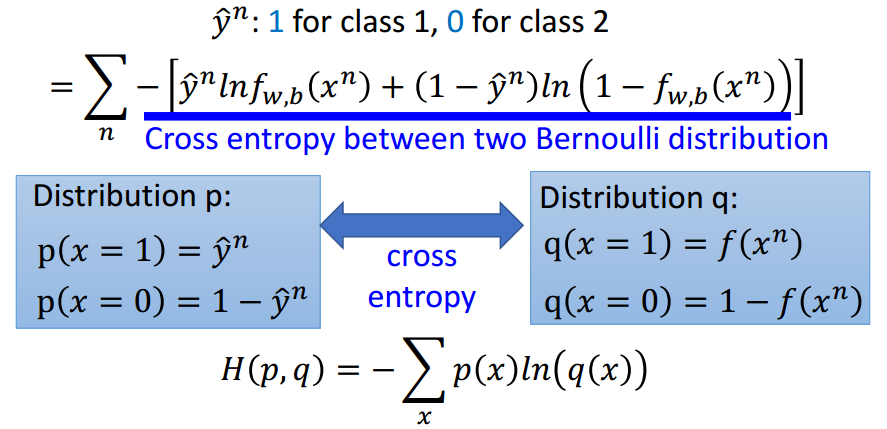
\includegraphics[scale=0.4]{pic/cross_entropy_bernoulli}
	\caption{交叉熵函数}
	\label{fig:cross_entropy}
\end{figure}
\begin{myquotation}{$\frac{\partial L}{\partial w_i}$推导}
	\[
	\frac{\partial L}{\partial w_i} = \sum_n -\hat{y}^n \frac{\partial \ln \sigma(z)}{\partial w_i} - (1-\hat{y}^n) \frac{\partial (\ln(1 - \sigma(z)))}{\partial w_i}
	\]

\[
\frac{\partial \ln \sigma(z)}{\partial w_i} = \frac{\partial \ln \sigma(z)}{\partial \sigma(z)} \frac{\partial \sigma(z)}{\partial z} \frac{\partial z}{w_i} = \frac{1}{\sigma z} \sigma(z) (1-\sigma(z)) x^n_i = (1-\sigma(z)) x^n_i
\]
\[
\frac{\partial \ln (1-\sigma(z))}{\partial w_i} = \frac{\partial \ln (1-\sigma(z))}{\partial \sigma(z)} \frac{\partial \sigma(z)}{\partial z} \frac{\partial z}{w_i} = -\frac{1}{1-\sigma(z)} \sigma(z) (1-\sigma(z)) x^n_i =- \sigma(z) x^n_i
\]
\[
\frac{\partial L}{\partial w_i} = \sum_n -\hat{y}^n (1-\sigma(z)) x^n_i - (1-\hat{y}^n) (- \sigma(z) x^n_i) == \sum_n (\sigma(z) - \hat{y}^n) x^n_i
\]
\[
w_{i+1} = w_i - \eta  \sum_n (\sigma(z) - \hat{y}^n) x^n_i
\]
其中,$\sigma '(z) = \sigma(z)(1- \sigma(z))$
\end{myquotation}

\subsection{逻辑回归与线性回归的对比}
逻辑回归和线性回归方法的三步骤对比如图\ref{fig:log_reg_vs_liner_reg}所示:
\begin{figure}[htb]
	\centering
	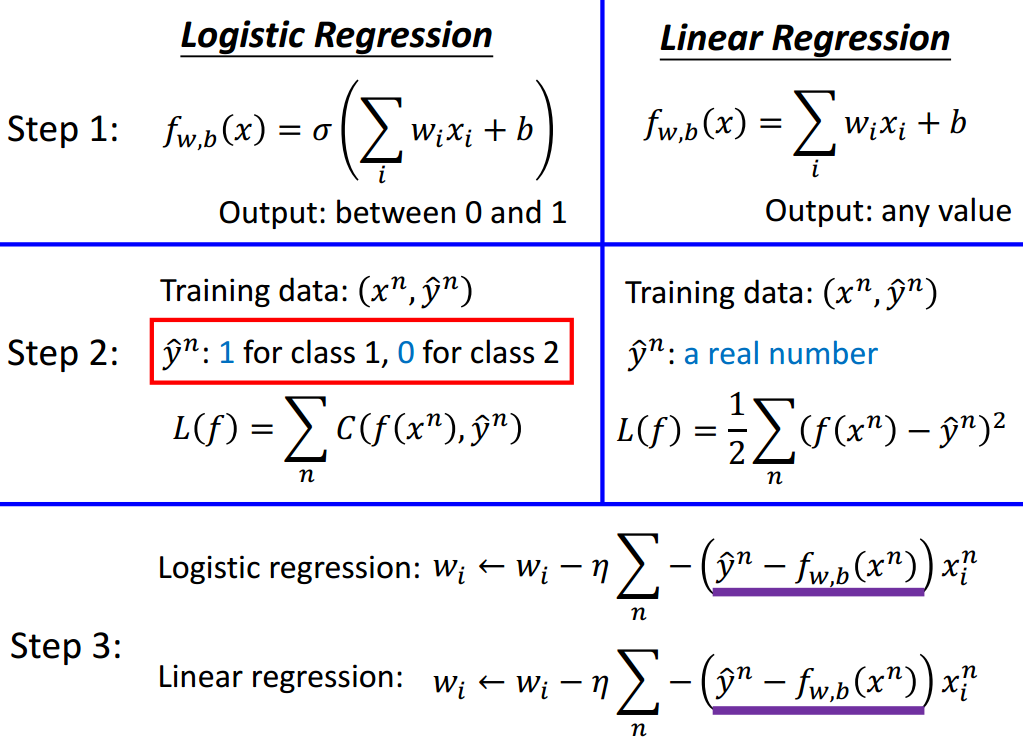
\includegraphics[scale=0.4]{pic/log_reg_vs_liner_reg}
	\caption{逻辑回归与线性回归的对比}
	\label{fig:log_reg_vs_liner_reg}
\end{figure}
可以看出就权重的迭代而言,方程是一样的。同时也有一个疑问,为什么逻辑回归的损失函数要选择复杂的交叉熵函数,而不是 square error 函数?解释如图\ref{fig:when_log_reg_using_square_error}:
\begin{figure}[htb]
	\centering
	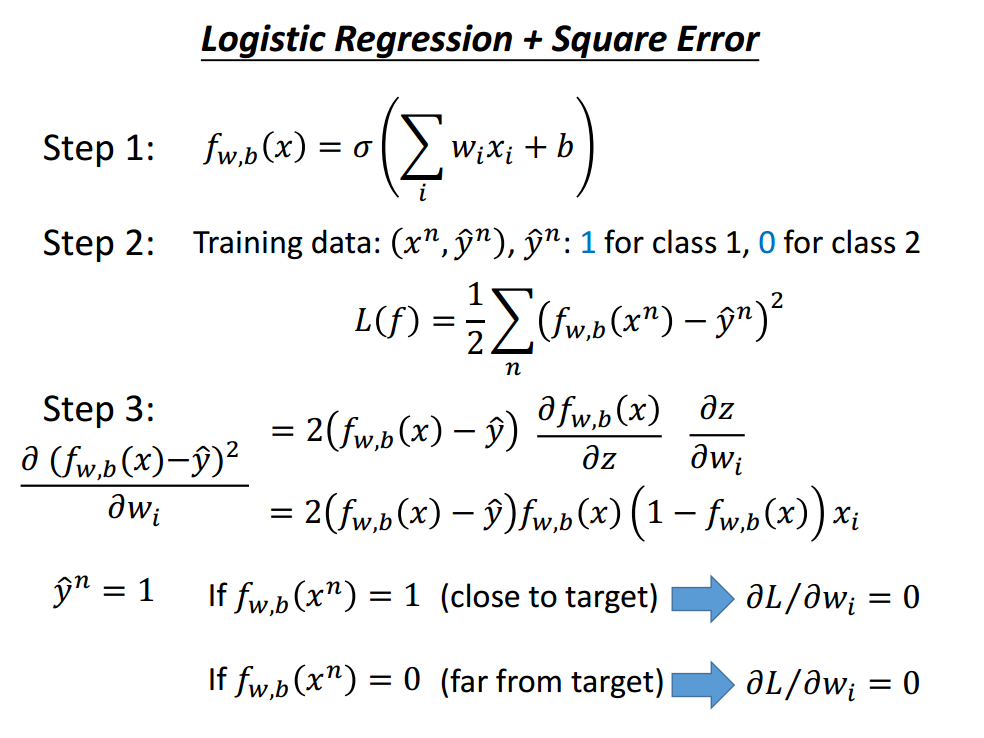
\includegraphics[scale=0.4]{pic/when_log_reg_using_square_error}
	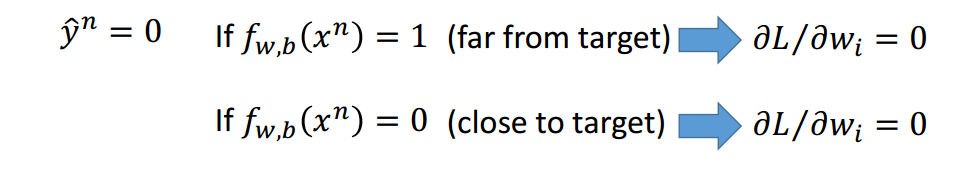
\includegraphics[scale=0.4]{pic/when_log_reg_using_square_error_02}
	\caption{逻辑回归的损失函数选择 square error 时发生了什么?}
	\label{fig:when_log_reg_using_square_error}
\end{figure}
可以看出,在$f_{w,b}(x)$在原理真值$\hat{y}^n$时,权重的偏导数就为0,因此,迭代停止。更为形象的比较见图\ref{fig:cross_entropy_vs_square_error}。
\begin{figure}[htb]
	\centering
	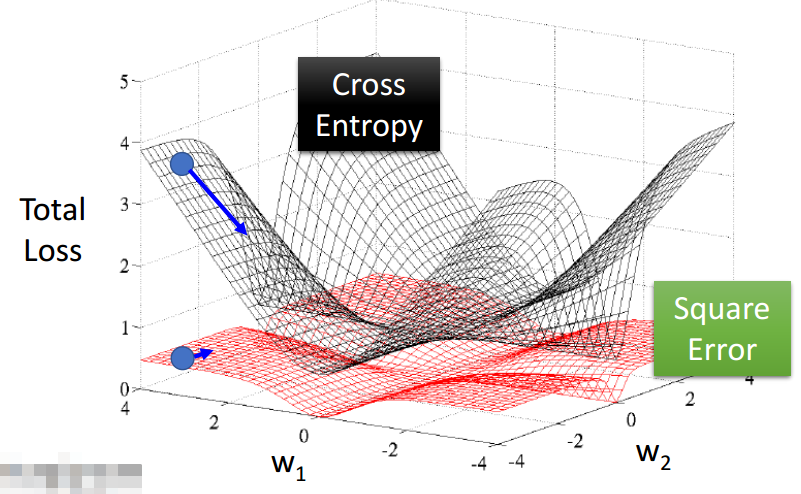
\includegraphics[scale=0.4]{pic/cross_entropy_vs_square_error}
	\caption{cross entropy vs square error}
	\label{fig:cross_entropy_vs_square_error}
\end{figure}

\subsection{多类别分类问题}
对于多分类问题,使用 softmax 函数解决,三类别问题如图所示\ref{fig:softmax}。首先通过训练不同的二分类判别模型,计算新样本在不同二分类模型下的输出$z_i=w_i x+b_i$,经过 softmax 函数,输出归于 0--1之间,判别新样本类别,样本的真是类别为 one hot 向量。输入向量与目标类别的损失函数定义为 cross entropy。

\begin{figure}
	\centering
	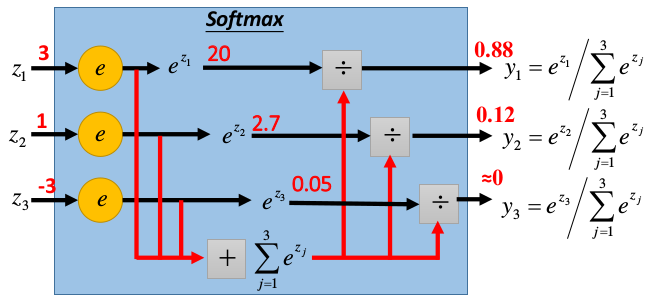
\includegraphics[scale=0.5]{pic/softmax}
	\caption{softmax}
	\label{fig:softmax}
\end{figure}

\subsection{逻辑回归的局限与深度学习的由来}
逻辑回归是一种线性分类方法,如图示数据,明显的使用线性模型无法分类。对原始特征进行相同的合理变换,就可以使用逻辑回归分类,而这种变换方法也可以通过逻辑回归模型实现。
\begin{figure}[htbp]
	\centering
	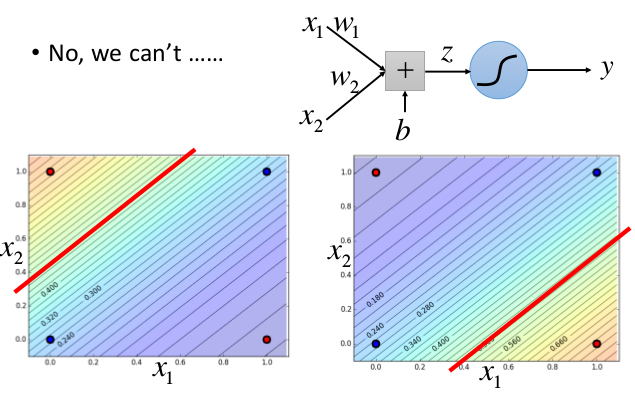
\includegraphics[scale=0.4]{pic/limition_log_reg}
	\caption{逻辑回归不能处理的数据}
	\label{fig:limition_log_reg}
\end{figure}
如图\ref{fig:transform_feature}所示,通过两个逻辑回归对二维特征进行变换,再使用一个逻辑回归模型进行分类。
\begin{figure}[htbp]
	\centering
	{\subcaptionbox{特征变换}{%
			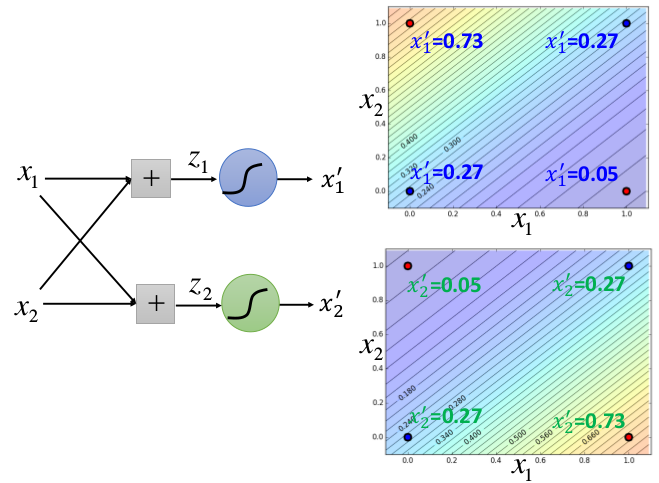
\includegraphics[scale=0.4]{pic/transform_feature_01}}\quad
	\subcaptionbox{分类}{%
	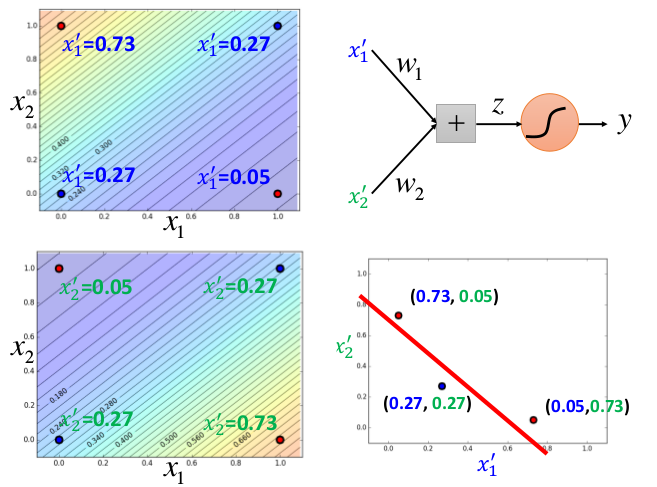
\includegraphics[scale=0.4]{pic/transform_feature_02}}
}
\caption{使用逻辑回归进行特征变换与分类}
\label{fig:transform_feature}
\end{figure}

深度学习的基本思想由此而来,通过前层对输入特征加以变换,最后使用 softmax 分类器分类。
\subsection{liner regression 其它推导方法}

对于线性回归模型 $y=\omega^T+b$ 输出的预测值 $y$ 都是实值,考虑二分类任务,$y_i\in\{0,1\}$。为了将实值 $y$ 对应到离散值,使用了 sigmoid 函数。如下:
\[
\mathrm{sigmoid:} \qquad y=\frac{1}{1+e^{-z}}=\frac{1}{1+e^{-(\omega^T+b)}}
\] 
对$\omega$和$b$作以下变换,令

\[
\beta=(\omega;b) \qquad \hat{x}=(x;1)
\]
则$y=\omega^T+b=\beta^T\hat{x}$,代入 sigmoid 函数。

\begin{equation}\label{sigmoid}
y=\frac{1}{1+e^{-\beta^T\hat{x}}}
\end{equation}
对 sigmoid 函数,$z=\ln\frac{y}{1-y}$,则式\eqref{sigmoid}可以变为

\begin{equation}\label{probability}
\ln\frac{y}{1-y}=\beta^T\hat{x}
\end{equation}
若将$y$视为类后验概率估计$P(y=1|x)$,即样本属于第一类的概率。则式\eqref{probability}可以写为:

\[
\ln\frac{P(y=1|x)}{1-P(y=1|x)}=\ln\frac{P(y=1|x)}{P(y=0|x)}=\beta^T\hat{x}
\]
对于样本集$\{x_i,y_i\}^{m}_{i=1}$,样本的概率可以写为:

\begin{equation*}
P(y_i|\beta;\hat{x_i})=P(y_i=1|\beta;\hat{x_i})^{y_i}\left(1-P(y_i=1|\beta;\hat{x_i})\right)^{1-y_i}
\end{equation*}
其中:

\begin{align}
P(y=1|x)&=\frac{e^{\beta^Tx}}{1+e^{\beta^Tx}}\\
P(y=0|x)&=\frac{1}{1+e^{\beta^Tx}}
\end{align}
n个独立的样本出现的似然函数为(因为每个样本都是独立的,所以n个样本出现的概率就是他们各自出现的概率相乘):

\begin{equation}
L(\theta)=\prod	P(y_i|\beta;\hat{x_i})
\end{equation}
对上式取对数,

\begin{equation}\label{siran}
\begin{split}
L(\theta)&=\log\prod	P(y_i|\beta;\hat{x_i})\\
&=\log \prod \left(P(y_i=1|\beta;\hat{x_i})^{y_i}\left(1-P(y_i=1|\beta;\hat{x_i})\right)^{1-y_i} \right)\\
&=\sum\log \left(P(y_i=1|\beta;\hat{x_i})^{y_i}\left(1-P(y_i=1|\beta;\hat{x_i})\right)^{1-y_i} \right)\\
&=\sum \left[ y_i\log P(y_i=1|\beta;\hat{x_i}) + (1-y_i)\log(1-P(y_i=1|\beta;\hat{x_i}))\right]\\
&=\sum \left( y_i \log P(y_i=1) - y_i \log(P(y_i=0))+\log(P(y_i=0))\right)\\
&=\sum \left( y_i \log \frac{P(y_i=1)}{P(y_i=0)} + log(\frac{1}{1+e^{\beta^T\hat{x_i}}})\right)\\
&=\sum \left(
y_i\beta^T\hat{x_i}-log(1+e^{\beta^T\hat{x_i}})
\right)
\end{split}
\end{equation}
为了优化求解,对目标函数取反,以进行最小值优化。对式\eqref{siran}	取反后,对$\beta$求导数:

\begin{equation}\label{key}
\begin{split}
\mathrm{d}L(\theta)
&=\sum \left(
\frac{e^{\beta^T\hat{x_i}} \mathrm{d}\beta^T\hat{x_i}}{1+e^{\beta^T\hat{x_i}} }
- y_i \mathrm{d} \beta^T \hat{x_i}
\right)\\
&=\mathrm{tr}\sum \left(
\frac{\hat{x_i}e^{\beta^T\hat{x_i}} \mathrm{d}\beta^T}{1+e^{\beta^T\hat{x_i}} }
- \hat{x_i}y_i \mathrm{d} \beta^T
\right)\\
&=\sum \hat{x_i}(P(y_i=1|\beta;\hat{x_i})-y_i)\mathrm{d}\beta^T
\end{split}
\end{equation}

\begin{equation*}
\frac{\partial \mathrm{d}L(\theta)}{\partial \beta^T}=\sum \hat{x_i}^T(P(y_i=1|\beta;\hat{x_i})-y_i)
\end{equation*}

\begin{equation}
\frac{\partial \mathrm{d}L(\theta)}{\partial \beta}=\sum \hat{x_i}(P(y_i=1|\beta;\hat{x_i})-y_i)
\end{equation}
运用梯度下降法进行优化求解:

\[
\beta_{n+1}=\beta_{n}-\alpha\frac{\partial \mathrm{d}L(\theta)}{\partial \beta}
\]
